
\chapter{Aufbau und Analyse der ETL Prozesse}

\section{Wettervorhersagen}

Wettervorhersagen haben das Ziel den Zustand der Erdatmosphäre zu
einer bestimmten Zeit an einem bestimmten Ort zu prognostizieren. Sie
werden meist von staatlichen oder privaten Wetterdiensten erstellt,
die sich an den Erkenntnissen der Meteorologie bedienen. Heutige
Wettervorhersagen basieren auf den aufwendig berechneten Ergebnissen
numerischer Wettermodelle.

Die Vorhersage des Wetters ist ein typisches Anfangswertproblem, das
meist in drei Schritten gelöst wird. Im ersten Schritt, der Analyse,
wird der Ausgangszustand der Atmosphäre bestimmt. Dieser Zustand wird
durch verschiedene physikalische Größen festgelegt, die von
Wetterstationen, Satelliten, Bojen oder Flugzeugen gemessenen
werden. Typische Größen repräsentieren dabei Luftdruck, Temperatur,
Wind, Wasserdampf, Wolken und Niederschlag.

Die Modellberechnung ist der zweite Schritt, und simuliert die
Entwicklung der Atmosphäre in die Zukunft. Die Berechnung dieser
Simulation ist sehr aufwendig, weshalb meist Supercomputer eingesetzt
werden. Ergebnis der Modellberechnung ist der Zustand der Atmosphäre
zu verschiedenen Zeitpunkten in der Zukunft, dargestellt durch
physikalischen Größen.

Im letzten Schritt, der Nachbereitung, werden die Ergebnisse der
Simulation schließlich für die verschiedensten Nutzer
aufbereitet. Dies beinhaltet die Generierung von Wetterkarten,
Warnhinweisen für Technisches Hilfswerk und Feuerwehr oder die
Visualisierung Strömungsfilmen.

\subsection{Numerische Wettermodelle}

Numerische Wettermodelle Modelle versuchen den Zustand der Atmosphäre
und deren Veränderung im Laufe der Zeit als mathematisches Problem zu
beschreiben. Dabei werden die physikalischen Größen und Beziehungen,
die den Zustand und die Veränderung der Atmosphäre beschreiben, als
System partieller Differentialgleichungen modelliert. Die meisten
Modelle verwenden dabei dieselben physikalischen Gesetzmäßigkeiten,
die auf den Erhaltungssätzen von Energie, Impuls und Masse
beruhen. Meist unterscheiden sie sich aber in der konkreten
mathematischen Formulierung und der numerischen Lösung der
Gleichungssysteme, weshalb die Ergebnisse verschiedener Modelle
erheblich voneinander abweichen können.

\subsubsection{Populäre Wettermodelle}

Der Deutsche Wetterdienst betreibt drei verschiedene
Wettermodelle. Die lokalen \textit{COSMO-DE} und \textit{COSMO-EU}
Modelle liefern Vorhersagen für Deutschland und Europa, das globale
Modell \textit{GME} hingegen Vorhersagen für die ganze Welt. Weitere
bekannte Modelle sind das von der US-amerikanischen \textit{National
  Oceanic and Atmospheric Administration} betriebene \textit{Global
  Forecast System (GFS)} \nomenclature{GFS}{Global Forecast System}
und das neuere \textit{Weather Research and Forecasting (WRF)}
\nomenclature{WRF}{Weather Research and Forecasting} Modell, das vom
\textit{National Weather Service (NWS)} \nomenclature{NWS}{National
  Weather Service}, vom amerikanischen Militär und einigen privaten
meteorologischen Organisationen verwendet wird.

\subsubsection{Diskretisierung von Raum und Zeit}

Um die sich verändernde Atmosphäre der Erde auf ein Modell abbilden zu
können wird eine Diskretisierung von Raum und Zeit vorgenommen. Dabei
wird die Oberfläche der Erde mit einem aus Drei- oder Vierecken
bestehenden Gitternetz überzogen, und die Atmosphäre vertikal in
mehrere Luftschichten aufgeteilt. Damit wird die unendlich Zahl der
möglichen Vorhersagepunkte in der Atmosphäre auf die endliche Zahl der
so entstandenen Kreuzungspunkte reduziert. In Abbildung
\ref{gitternetz} ist das dreieckige Gitternetz des zur Zeit vom
Deutschen Wetterdienst und des Max-Planck-Instituts für Meteorologie
neu entwickelten \textit{ICON} \nomenclature{ICON}{ICOsahedral
  Non-hydrostatic General Circulation Model} Wettermodells zu sehen.

\begin{figure}[h]
  \begin{center}
    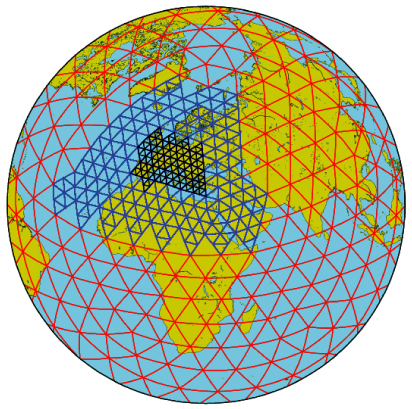
\includegraphics[height=200px]{bilder/gitternetz}
    \caption{Dreiecksgitter des ICON Wettermodells}
    \label{gitternetz}
  \end{center}
\end{figure}

Mit der Maschenweite bezeichnet man den horizontalen Abstand zwischen
zwei benachbarten Gitterpunkten. Je feiner das Gitter, bzw. je höher
die Auflösung des Modells ist, desto genauer kann die Erdoberfläche
und die darüber liegenden atmosphärischen Strukturen erfasst werden,
was sich auf die Genauigkeit der Wettervorhersage auswirkt. Die
benötigten Ressourcen zu Berechnung der Modellgleichungen steigt mit
der Anzahl der verwendeten Gitterpunkte.

Da eine sehr hohe Auflösungen selbst die Leistungsfähigkeit der
schnellsten Supercomputer übersteigt werden von den Wetterdiensten
meist verschiedene Modelle in unterschiedlichen Auflösungen
berechnet. Globale, den gesamten Globus umfassende Modelle werden mit
einer geringeren Auflösung als lokale, Länder oder Kontinente
abdeckende Modelle berechnet. Je weiter in die Zukunft prognostiziert
werden soll, desto mehr spielen aber wieder Wetterphänomene aus
Gebieten die nicht vom lokalen Modell abgedeckt werden eine Rolle. Für
Vorhersagen ab 5 Tagen in die Zukunft benötigen die lokalen Modelle
wiederum Informationen aus der gesamten Atmosphäre. Deshalb verwenden
die höher auflösenden lokalen Modelle oft Informationen als Randwerte
aus den zuvor berechneten globalen Modelle.

Die zeitliche Diskretisierung hingegen ist weniger problematisch. Die
meisten Modelle bieten mindestens Prognosen um 12 und 24 Uhr für
diejenigen Tage an, über die sich der Vorhersagezeitraum
erstreckt. Das \textit{Global Forecast System} Modell berechnet die
Vorhersagen beispielsweise im drei Stunden Intervall.

\section{Überblick der verwendeten Datenquellen}

\subsection{Global Forecast System}
\subsection{Wave Watch III}

% Die Erde umgebende Atmosphäre wird
% in numerischen Wettermodelle in


% , die von verschiedenen
% Wetterdiensten erstellt und betrieben werden.

% \subsection{Wetter- und Wellendaten}

%  Diese Modelle versuchen
% den Zustand der Atmosphäre und deren Veränderung als mathematisches
% Problem zu berschreiben. Eingabe für ein solches Modell ist der
% Zustand der Atmosphäre in Form von physikalischen Größen, wie
% z.B. Temperatur, Windstärke und Windrichtung. Die physikalischen
% Beziehungen, die den Zustand der Atmosphäre verändern werden als
% System partieller Differentialgleichungen modelliert.

% Verfahren der Numerik
% und der Einsatz von Supercomputern helfen dabei d


% formuliert. Zur Lösung des Problems werden Verfahren

% Dieses wird mit Verfahren der Numerik und dem Einsatz von
% Supercomputern näherungsweise gelöst. Das Ergebnis

% Es gibt eine Vielzahl dieser Modelle die
% von unterschiedlichen Wetterdiensten erstellt werden, und aufgrund der
% Anwendung verschiedener Verfahren auch erhebliche Abweichungen



% Diese Ergebnisse repräsentieren
% den Zustand der Atmosphäre für ein Vorhersagegebiet zu einem
% bestimmten Zeitpunkt in Form von physikalischen Größen, wie
% z.B. Temperatur, Windstärke und Windrichtung.



% Diese E



% Das Vorhersagegebiet wird dabei in Gitterzellen


%  als dreidimensionaler Raum in
% Abhängigkiet der Zeit betrachtet.

% in Gitterzellen aufgeteilt, um die für
% das Modell relevanten physikalischen Größen als Funktion der Zeit im
% dreidimensionalen Raum darstellen zu können.

% .System


%  in Form
% von partiellen Differentialgleichungen dar.


% Die Berechnung dieser
% Modelle ist sehr aufwendig, weshalb Verfahren aus dem Bereich der
% Numerik und Supercomputer verwendet werden um das Problem
% näherungsweise zu lösen.

% Der Zustand der Atmosphäre


% . Dieser
% dreidimensionale Raum wird durch die geographischen Koordinaten
% Latitude, Longitude sowie der Höhe über dem Meeresspiegel aufgespannt.

% Die Eckpunkte
% einer Gitterzelle representieren dabei die physikalischen Größen wie
% z.B. Temperatur, Windrichtung und -stärke, Wellenhöhe und
% -periode sind einige der






% , wie Temperatur,
% Luftdruck, Windrichtung, Windstärke, etc.

% Problem zu formulieren.

% , und durch die Lösung darzustellen.

% System partieller
% Differentialgleichungen darzustellen.


% zu einem gegeben Zeitpunkt durch die
% numerische Lösung


% Es gibt eine Vielzahl von
% Wettermodellen die von verschiedenen Wetterdiensten für bestimmte
% Regionen angeboten werden.


% Für die Berechnung dieser Modelle
% wird ein Gebiet oder Region in Gitterzellen aufgeteilt.


% Es gibt eine Vielzahl dieser
% Modelle,


% In einem solchen Modell wir das


% , die sind rechnergestützte Wettervorhersagen

% Die für die Wetter- und Wellenvorhersagen benötigten Daten werden von
% der US-amerikanischen Wetter- und Ozeanografiebehörde \textit{National
%   Oceanic and Atmospheric Administration (NOAA)} als Ergebnis
% numerisch gelöster Wettermodelle zur Verfügung gestellt.

\subsection{Photos \& Videos}
\section{Datenbank Design}
\subsection{Konzeptionelle Schema}
\subsection{Physisches Schema}
\section{Extraktion aus den Quellsystemen}
\section{Transformation der Daten}
\section{Laden der Daten}
\section{Verbesserungen}

%%% Local Variables:
%%% mode: latex
%%% TeX-master: "../community-plattform"
%%% End:
